\documentclass[11pt]{article}
\usepackage[a4paper,margin=21mm]{geometry}
\usepackage{amsmath,amssymb,booktabs,array}
\usepackage{tikz}
\usepackage[T1]{fontenc}
\usepackage{lmodern}
\usepackage[hidelinks]{hyperref}
\usepackage{listings}
\lstset{basicstyle=\ttfamily\small,breaklines=true,columns=fullflexible,frame=single}
\setlength{\parindent}{0pt}
\setlength{\parskip}{6pt}
\setlength{\emergencystretch}{1.5em}
\newcommand{\mos}[4]{\begin{scope}[shift={(#1,#2)}]
\draw (0,.24)--(0,-.24);
\draw (0,.20)--(.25,.20)--(.25,.5);
\draw (0,-.20)--(.25,-.20)--(.25,-.5);
\draw (-.16,.23)--(-.16,-.23);
\ifnum#4=1\draw (-.26,0) circle (.06);\draw (-.75,0)--(-.32,0);\else\draw (-.75,0)--(-.16,0);\fi
\node[anchor=east,font=\small] at (-.76,0) {$#3$};
\end{scope}}
\newcommand{\ground}[2]{\draw (#1,#2)--(#1,{#2-.12});\draw ({#1-.17},{#2-.12})--({#1+.17},{#2-.12});\draw ({#1-.11},{#2-.20})--({#1+.11},{#2-.20});}
\newcommand{\rail}[3]{\draw (#1,#2)--(#1,{#2+.15});\node[above,font=\small] at (#1,{#2+.15}) {$#3$};}
\newcommand{\outputnode}[3]{\fill (#1,#2) circle (.04);\draw (#1,#2)--({#1+.7},#2) node[right] {$#3$};}
\begin{document}
\begin{center}{\Large\bfseries Introduction to VLSI Design, 2015}\par{\large Homework 1: complete theory and CMOS solution}\end{center}
The original PDF, rather than OCR, determines the expressions. Q4(a) has an outer complement over the full expression and a second complement over $(x+y)$.

\section*{1. Which inverter transistors cannot saturate?}
$M_1$ is the grounded NMOS, $M_2$ the NMOS near the output; $M_4$ is the PMOS adjacent to $V_{DD}$ and $M_3$ the PMOS near the output. Let $u$ be the NMOS internal node and $v$ the PMOS internal node. All gates use $V_{in}$. Neglect body effect as specified.

\begin{center}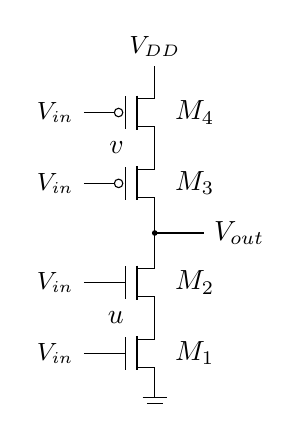
\begin{tikzpicture}[scale=.9]
\mos{0}{0}{V_{in}}{0}\mos{0}{1}{V_{in}}{0}\mos{0}{2.4}{V_{in}}{1}\mos{0}{3.4}{V_{in}}{1}
\draw (.25,1.5)--(.25,1.9);\outputnode{.25}{1.7}{V_{out}}\rail{.25}{3.9}{V_{DD}}\ground{.25}{-.5}
\node[right] at (.4,0){$M_1$};\node[right] at (.4,1){$M_2$};\node[right] at (.4,2.4){$M_3$};\node[right] at (.4,3.4){$M_4$};
\node[left] at (-.05,.5){$u$};\node[left] at (-.05,2.9){$v$};
\end{tikzpicture}\end{center}
If $M_1$ saturates, $u\ge V_{in}-V_{tn}$. Then $V_{GS,2}=V_{in}-u\le V_{tn}$ and $M_2$ cannot carry nonzero current. Hence a conducting $M_1$ must be linear. Similarly, $M_4$ saturation implies $v\le V_{in}+|V_{tp}|$, giving $V_{SG,3}=v-V_{in}\le|V_{tp}|$ and switching off $M_3$. Thus
\[
\boxed{M_1\text{ and }M_4\text{ cannot saturate while their series paths conduct.}}
\]
$M_2$ and $M_3$ can saturate. This statement concerns nonzero conduction, not a cutoff device classified using inequalities alone.

\section*{2. Series-channel equivalence: complete derivation}
Let the bottom NMOS have length $L_2$, the top NMOS length $L_1$, common width $W$, common threshold $V_t$, and gate voltage $V_G$. Set the external source to 0 and drain to $V_D$; the internal node is $u$. Define $k=\mu_n C_{ox}W$ and $a=V_G-V_t$. When both devices are linear,
\begin{align*}
I L_2/k&=au-u^2/2,\\
I L_1/k&=(a-u)(V_D-u)-(V_D-u)^2/2.
\end{align*}
Adding cancels the internal node:
\[
\boxed{I=\frac{k}{L_1+L_2}\left(aV_D-\frac{V_D^2}{2}\right).}
\]
This is exactly the long-channel linear current of a single transistor with $W/(L_1+L_2)$. If the upper transistor saturates, replace its equation by $I L_1/k=(a-u)^2/2$; adding the lower equation gives $I=k a^2/[2(L_1+L_2)]$, the corresponding saturation current. For $L_1=L_2=L$, the equivalent device has width $W$ and length $2L$. Common thresholds, no body effect, and the ideal square-law model are essential. The equivalence does not preserve internal diffusion capacitance or physical transient delay.

\newpage\section*{3. One 4-to-1 MUX implementation}
The required function is $F=\bar A(B+\bar C)+A\bar BC$. Choose $A,B$ as the select bits, with $A$ the most significant bit. The Shannon cofactors are
\begin{center}\begin{tabular}{cc|c}\toprule $A$&$B$&Data input\\\midrule
0&0&$D_0=\bar C$\\0&1&$D_1=1$\\1&0&$D_2=C$\\1&1&$D_3=0$\\\bottomrule\end{tabular}\end{center}
Thus $F=\operatorname{MUX4}(A,B;\bar C,1,C,0)$. If $\bar C$ is unavailable, generate it with a CMOS inverter (2 extra MOSFETs).
\begin{center}\begin{tikzpicture}
\draw (0,0) rectangle (2,3.2);\node at (1,1.6){4:1 MUX};
\foreach \y/\lab in {.4/0,1.2/C,2/1,2.8/\bar C}{\draw (-1,\y)--(0,\y) node[pos=0,left]{$\lab$};}
\draw (.7,-.6)--(.7,0) node[pos=0,below]{$A$};\draw (1.3,-.6)--(1.3,0) node[pos=0,below]{$B$};\draw (2,1.6)--(3,1.6) node[right]{$F$};
\node[right,font=\small] at (3.5,1.6){$D_0$ at top, $D_3$ at bottom};
\end{tikzpicture}\end{center}
\begin{center}\begin{tabular}{ccc|c}\toprule $A$&$B$&$C$&$F$\\\midrule
0&0&0&1\\0&0&1&0\\0&1&0&1\\0&1&1&1\\1&0&0&0\\1&0&1&1\\1&1&0&0\\1&1&1&0\\\bottomrule\end{tabular}\end{center}

\newpage\section*{4(a). Double-bar static CMOS function}
The visually confirmed expression is
\[
\boxed{f=\overline{w\,\overline{(x+y)}+yz}.}
\]
Generate $t=\overline{x+y}$ with a NOR gate (4 MOSFETs). Then a static AOI22 gate forms $f=\overline{wt+yz}$ using 8 more MOSFETs. No complemented external literal is required. The NOR PDN is $n_x\parallel n_y$ and its PUN is $p_x$ in series with $p_y$. The AOI22 PDN has $(n_w,n_t)$ and $(n_y,n_z)$ series branches in parallel; its PUN is $(p_w\parallel p_t)$ in series with $(p_y\parallel p_z)$.

\begin{center}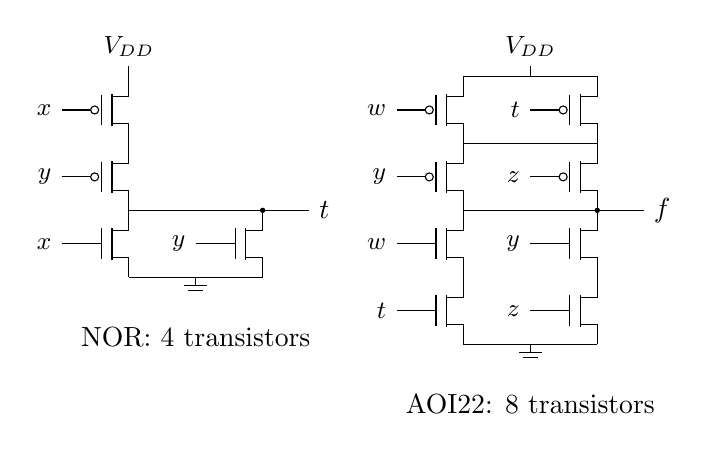
\begin{tikzpicture}[scale=.85]
% NOR for t
\mos{0}{4}{x}{1}\mos{0}{3}{y}{1}\rail{.25}{4.5}{V_{DD}}
\draw (.25,2.5)--(2.25,2.5);\outputnode{2.25}{2.5}{t}
\mos{0}{2}{x}{0}\mos{2}{2}{y}{0}\draw (.25,1.5)--(2.25,1.5);\ground{1.25}{1.5}
\node[below] at (1.25,.9){NOR: 4 transistors};
% AOI22
\mos{5}{4}{w}{1}\mos{7}{4}{t}{1}\draw (5.25,4.5)--(7.25,4.5);\rail{6.25}{4.5}{V_{DD}}
\mos{5}{3}{y}{1}\mos{7}{3}{z}{1}\draw (5.25,3.5)--(7.25,3.5);\draw (5.25,2.5)--(7.25,2.5);\outputnode{7.25}{2.5}{f}
\mos{5}{2}{w}{0}\mos{5}{1}{t}{0}\mos{7}{2}{y}{0}\mos{7}{1}{z}{0}\draw (5.25,.5)--(7.25,.5);\ground{6.25}{.5}
\node[below] at (6.25,-.1){AOI22: 8 transistors};
\end{tikzpicture}\end{center}
The intermediate $t$ is the signal joining the two diagrams. PMOS body terminals connect to $V_{DD}$, NMOS bodies to ground. Total device count is 12. For all 16 true-input combinations, each CMOS stage has exactly one conducting pull-up or pull-down network.

\newpage\section*{4(b). Anti-majority static CMOS function}
For $f=\bar x\bar y+\bar x\bar z+\bar y\bar z$, use
\[
\bar f=(x+y)(x+z)(y+z)=xy+xz+yz.
\]
The PDN is three series stages of two parallel NMOS devices. The PUN is its dual: three parallel branches of two series PMOS devices. Gate labels use only true inputs; repeated labels are separate devices. This direct construction has 12 transistors.
\begin{center}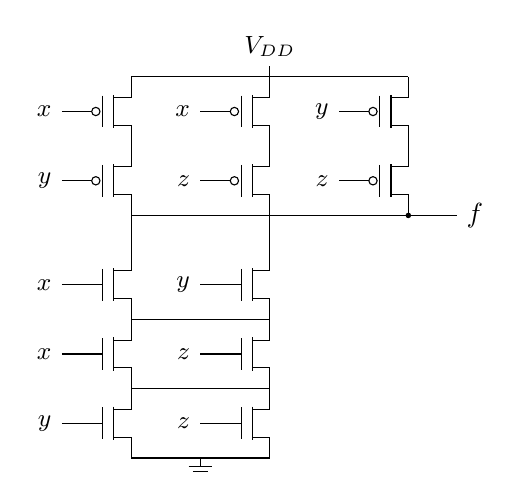
\begin{tikzpicture}[scale=.88]
\mos{0}{4}{x}{1}\mos{0}{3}{y}{1}\mos{2}{4}{x}{1}\mos{2}{3}{z}{1}\mos{4}{4}{y}{1}\mos{4}{3}{z}{1}
\draw (.25,4.5)--(4.25,4.5);\rail{2.25}{4.5}{V_{DD}}\draw (.25,2.5)--(4.25,2.5);\outputnode{4.25}{2.5}{f}
\draw (.25,2.5)--(.25,2);\draw (2.25,2.5)--(2.25,2);
\mos{0}{1.5}{x}{0}\mos{2}{1.5}{y}{0}\mos{0}{.5}{x}{0}\mos{2}{.5}{z}{0}\mos{0}{-.5}{y}{0}\mos{2}{-.5}{z}{0}
\draw (.25,1)--(2.25,1);\draw (.25,0)--(2.25,0);\draw (.25,-1)--(2.25,-1);\ground{1.25}{-1}
\end{tikzpicture}\end{center}
\section*{Source review and checks}
Both supplied handwritten JPGs were inspected. Their $M_1/M_4$ answer and series-current elimination agree with Q1/Q2. Their 4-to-1 MUX table agrees with Q3. The drawn NOR intermediate plus CMOS network matches Q4(a); the rewritten algebra in the scan is less clear than the original PDF's two overbars, so the circuit was independently checked against the original expression. The Q4(b) diagram is retained as a valid direct dual network.

Run \texttt{python verify\_logic.py}. All 8 MUX, 16 Q4(a), and 8 Q4(b) combinations pass in \path{truth_tables.csv}. These are exhaustive Boolean conduction checks, not electrical simulation.

\end{document}
